\documentclass[a4paper,11pt,spanish,sans]{exam}
\usepackage[spanish]{babel}
%\usepackage[utf8]{inputenc}
\usepackage{multicol}
%\usepackage[latin1]{inputenc}
\usepackage{fontspec}%la posta para las tildes con lualatex
\usepackage[margin=0.5in]{geometry}
\usepackage{amsmath,amssymb}
\usepackage{natbib}
\usepackage{graphicx}
\usepackage{hyperref}
\usepackage{epstopdf}
\usepackage{capt-of}
\usepackage{gensymb}
\usepackage{float}
\usepackage{wrapfig}
\usepackage{pst-fractal}
%\usepackage{animate}
\usepackage[usenames]{color}
%para graficos
\usepackage{pgf,tikz}
\usepackage{mathrsfs}
\usetikzlibrary{arrows}
\usepackage{pst-fractal}
\usetikzlibrary{decorations.markings}
\usetikzlibrary{shapes.geometric}
\usetikzlibrary{shapes,snakes}
\usepackage{tkz-euclide}
\usetkzobj{all}

%\usepackage{pgfplots}  plots

%los de aca abajo capaz no los uso
\newcommand{\class}{Matemática: Guía de  Trigonometria} %Episodio IV una nueva esperanza (Guia 1).  %Episodio V: Las funciones contratacan (Guia 2).
\newcommand{\term}{3° Trimestre 2015}
\newcommand{\examnum}{}
\newcommand{\examprof}{Alexis Gomel}
\newcommand{\examdate}{15/7/2015}
\newcommand{\timelimit}{60 Minutes}%no lo uso
\newcommand{\webpdf}{https://drive.google.com/file/d/0B2MOYme4kZd-eS0zUFhNQjV6eUE/view?usp=sharing}%no lo uso
\newcommand{\Ts}{\rule{0pt}{2.6ex}}       % Top strut
\newcommand{\Bs}{\rule[-1.2ex]{0pt}{0pt}} % Bottom strut


%el header de las hojas.
\pagestyle{head}
\firstpageheader{}{}{}
\runningheader{\class}{\examnum\ - Pagina \thepage\ de \numpages}{\examterm}
\runningheadrule

\begin{document}

\noindent
\begin{tabular*}{\textwidth}{l @{\extracolsep{\fill}} r @{\extracolsep{6pt}} l}
\textbf{\class} & \textbf{Profesor: \examprof}\\

\textbf{PDF: \href{\webpdf}{\textcolor{blue}{http://tinyurl.com/Trigonometricas}}} %& Teaching Assistant & \makebox[2in]{\hrulefill}
\end{tabular*}\\
\rule[2ex]{\textwidth}{2pt}

%%%%%%%%%%%%%%%%%%%%%%%%%%%%%%%%%%%%%%%%%%%
%Temas: 


{{\small Esta guía es simplemente una guía. \textbf{\underline{NO} reemplaza ni incluye todo el material que se da en clase}}}.

\begin{center}
\section*{Guía de Funciones Trigonométricas}
\end{center}


Las funciones trigonométricas son aquellas en las que el argumento de la función (\textquotesingle$x$\textquotesingle) es un angulo.

Vamos a ver que esta familia de funciones son muy importantes en la geometría y para describir problemas de toda índole.%arreglar esto.

\section*{Sistema de medición de ángulos}

Existen 3 sistemas en los cuales se pueden medir los ángulos.\\
\textbf{ Sistema Sexagesimal}: La unidad básica es 1$\degree$. 

Un circulo completo tiene $360\degree$, un grado tiene ($60'$) minutos sexagesimales y un minuto sexagesimal ($1'$) tiene ($60''$) segundos sexagesimales.

Al igual que con el sistema métrico, existen subdivisiones mas pequeñas que el segundo sexagesimal, y su uso es frecuente en áreas como la astronomía donde una diferencia en inclinación menos de un segundo de arco en un telescopio puede ser cientos de miles de kilómetros de diferencia en el objeto que se quiere observar.

\textbf{Sistema Centesimal}: La unidad básica es 1 grado centesimal. y se define dividiendo un angulo recto en 100 partes iguales.

Por lo tanto un circulo completo tiene 400 grados centesimales, y se define que un grado tiene ($100'$) minutos centesimales y un minuto centesimal ($1'$) tiene ($100''$) segundos centesimales.

\textbf{Sistema circular}: La unidad básica es un radian ($1$) radian.
\begin{wrapfigure}{r}{0.2\textwidth}
  \begin{center}
    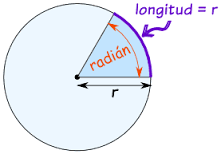
\includegraphics[width=\linewidth]{radian.png}
  \end{center}
\end{wrapfigure}
Los radianes no llevan un símbolo para identificarlos, y son MUY utilizados en el área científica como la forma mas común de medir ángulos a la hora de hacer cuentas.

Se llama radian al angulo que abarca un arco de circunferencia cuya longitud es igual al radio de la misma.


Por lo tanto, un circulo completo es un giro de ($2\pi $) radianes. Medio circulo ($180$) son $\pi$ radianes, un angulo recto son $\pi /2$ radianes, y así.

Vamos a ver que muchas veces los radianes son la forma mas cómoda para medir los ángulos.

\section*{Razones trigonométricas. Triangulo Rectángulo}

Pequeño repaso:
la suma de los ángulos internos de un triangulo suman $180\degree$.\\


\begin{minipage}{0.45\linewidth}

\begin{tikzpicture}[thick]
	\coordinate (O) at (0,0);
	\coordinate (A) at (3,0);
	\coordinate (B) at (0,4);
	\draw (O)--(A)--(B)--cycle;
	
	\tkzLabelSegment[below=2pt](O,A){\textit{C.adyacente }($b$)}
	\tkzLabelSegment[left=2pt](O,B){\textit{C. Opuesto }($a$)}
	\tkzLabelSegment[above right=2pt](A,B){\textit{hipotenusa }($h$)}
	
	\tkzMarkRightAngle[fill=orange,size=0.6,opacity=.4](A,O,B)% square angle here
	\tkzLabelAngle[pos = 0.35](A,O,B){$\hat{\gamma}$}
	
	\tkzMarkAngle[fill= orange,size=0.8cm,%
	opacity=.4](B,A,O)
	\tkzLabelAngle[pos = 0.6](B,A,O){$\hat{\alpha}$}
	
	\tkzMarkAngle[fill= orange,size=0.8cm,%
	opacity=.4](O,B,A)
	\tkzLabelAngle[pos = 0.5](O,B,A){$\hat{\beta}$}

\end{tikzpicture}

\end{minipage}
\begin{minipage}{0.5\linewidth}
Teorema de pitagoras:
\[
a^2+b^2=h^2
\]

Hay tres razones trigonométricas principales que se definen como: %cambiar
\[
\sin(\hat{\alpha})=\frac{\text{Cateto opuesto}}{hipotenusa}= \frac{a}{h}\]
\[
\cos(\hat{\alpha})=\frac{\text{Cateto adyacente}}{hipotenusa}=\frac{b}{h}
\]
\[
\tan(\hat{\alpha})=\frac{\text{Cateto opuesto}}{\text{Cateto adyacente}}=\frac{a}{b}
\]
\end{minipage}

Notar que lo que definimos como cateto opuesto o adyacente, depende del angulo que estemos usando ($\alpha$ en este caso).

Para $\beta$ el lado opuesto seria $b$ y el adyacente $a$.\\

Las funciones como el seno o el coseno son muy importantes en una cantidad enorme de aplicaciones y modelos.

Las funciones trigonométricas fueron usadas ya por los antiguos griegos para deducir que la tierra era redonda, y calcular aproximadamente su radio. 
Hasta en la actualidad para calcular la posición de las cosas con los GPS, la posición de los satélites, o incluso la posición de los jugadores de fútbol cuando muestran una repetición por la tele.

También son muy importantes en muchos modelos de naturaleza, por ejemplo el sonido o la luz, que se comportan como ondas, se modelan con senos y cosenos.

Incluso son necesarios para entender como tecnologías como los cassetes y los vinilos hasta los Blurays graban su información, o como funcionan las emisiones de la radio o los rayos x.

Describir como oscila un péndulo o como rebota un resorte también da como resultado un seno o un coseno.

\textbf{Uso de la calculadora:} Antes de empezar a hacer cuentas con la calculadora hay que tener cuidado y ponerla en el modo \textbf{DEG}(sexagesimal) o el modo \textbf{RAD}(radial), para que la calculadora entienda que los valores que estamos usando  están en unidades de grados o radianes, según corresponda.\\

\section*{Teoremas del seno y coseno}

\begin{minipage}{0.5\linewidth}

\begin{tikzpicture}[thick]
	\coordinate (O) at (0,0);
	\coordinate (A) at (3.5,0);
	\coordinate (B) at (-1,3);
	\draw (O)--(A)--(B)--cycle;
	
	\node at (O) [below left=2pt]{$a$};
	\node at (A) [right=2pt]{$b$};
	\node at (B) [above left=2pt]{$c$};
	
	\tkzLabelSegment[below=2pt](O,A){}
	\tkzLabelSegment[left=2pt](O,B){}
	\tkzLabelSegment[above right=2pt](A,B){}
	
	\tkzMarkAngle[fill=orange,size=0.6,opacity=.4](A,O,B)% square angle here
	\tkzLabelAngle[pos = 0.35](A,O,B){$\hat{a}$}
	
	\tkzMarkAngle[fill= orange,size=0.8cm,%
	opacity=.4](B,A,O)
	\tkzLabelAngle[pos = 0.6](B,A,O){$\hat{b}$}
	
	\tkzMarkAngle[fill= orange,size=0.7cm,%
	opacity=.4](O,B,A)
	\tkzLabelAngle[pos = 0.5](O,B,A){$\hat{c}$}
\end{tikzpicture}

\end{minipage}
\begin{minipage}{0.5\linewidth}
\textbf{Teorema del seno}:

\[
\frac{\overline{ab}}{\sin(\hat{c})}=\frac{\overline{ac}}{\sin(\hat{b})}=\frac{\overline{bc}}{\sin(\hat{a})}
\]

\href{http://tube.geogebra.org/material/simple/id/55239}{\textcolor{blue}{Versión interactiva del teorema del seno.}}

\textbf{Teorema del coseno}:

\[
\overline{ab}^2=\overline{ac}^2 + \overline{bc}^2 - 2.\overline{bc}.\overline{ac}.\cos(\hat{c})
\]

Se puede ver que el teorema de pitagóricas es un caso particular del \href{http://tube.geogebra.org/material/simple/id/3498}{\textcolor{blue}{teorema del coseno}}: si  $c=90 \degree$.

Así como el teorema vale para $\overline{ab}$, es igual de valido para $\overline{ac}$ y $\overline{bc}$, reescribiéndolo de la manera adecuada. 

\end{minipage}

\section*{Seno y Coseno en la circunferencia unitaria}

Empezando por el seno y el coseno: Pensemos en un circulo de radio $1$.

\begin{minipage}{0.45\linewidth}
	Como se ve en la figura, Para cada punto \textquotesingle$C$\textquotesingle de la circunferencia podemos dibujar un triangulo rectángulo.
	
	Entonces vamos a redefinir a el $\cos(\alpha)$ como el valor en el eje x del punto, y a el $\sin(\alpha)$ como el valor en el eje y del punto que elegimos en la circunferencia.  
	
	Para entender mejor esto pueden ver esta \href{http://tube.geogebra.org/m/960}{\textcolor{blue}{versión interactiva de seno y coseno, como componentes de un triangulo rectángulo en un circulo}}.

\end{minipage}
\begin{minipage}{0.55\linewidth}
	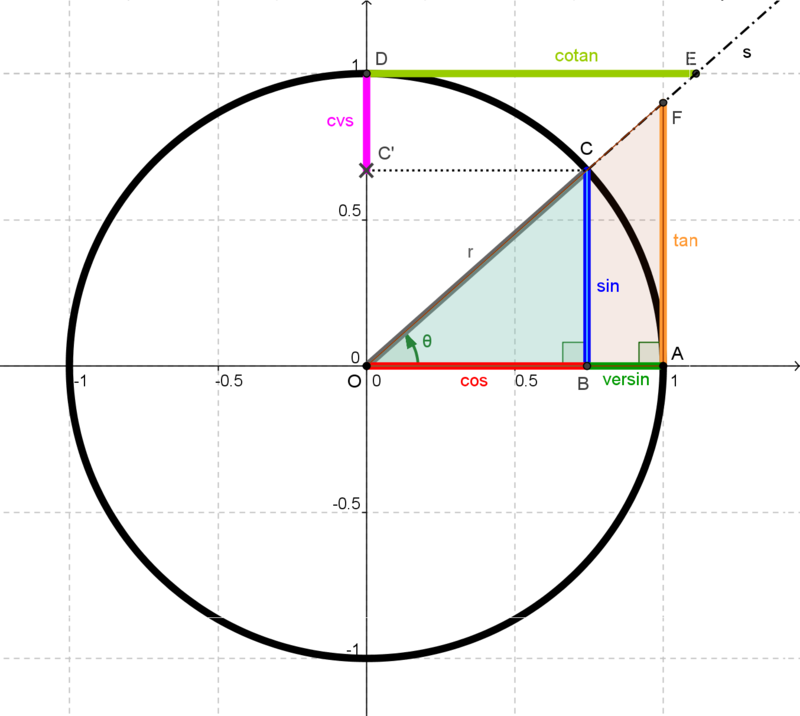
\includegraphics[width=0.85\textwidth]{trigocirc.png}
\end{minipage}

\section*{Gráficos de funciones trigonométricas}


Entonces si vemos cuanto valen el seno y el coseno \href{http://tube.geogebra.org/material/simple/id/311963}{\textcolor{blue}{a medida que recorremos la circunferencia unidad}} :


\begin{minipage}{0.3\linewidth}
	\[ y=\sin (x)\\
	
	\begin{cases}
		Dom(\sin (x))= x \in \mathbb{R} \\ 
		Im(\sin (x))= [-1,1]\\
	\end{cases} \]

\end{minipage}
\begin{minipage}{0.7\linewidth}
	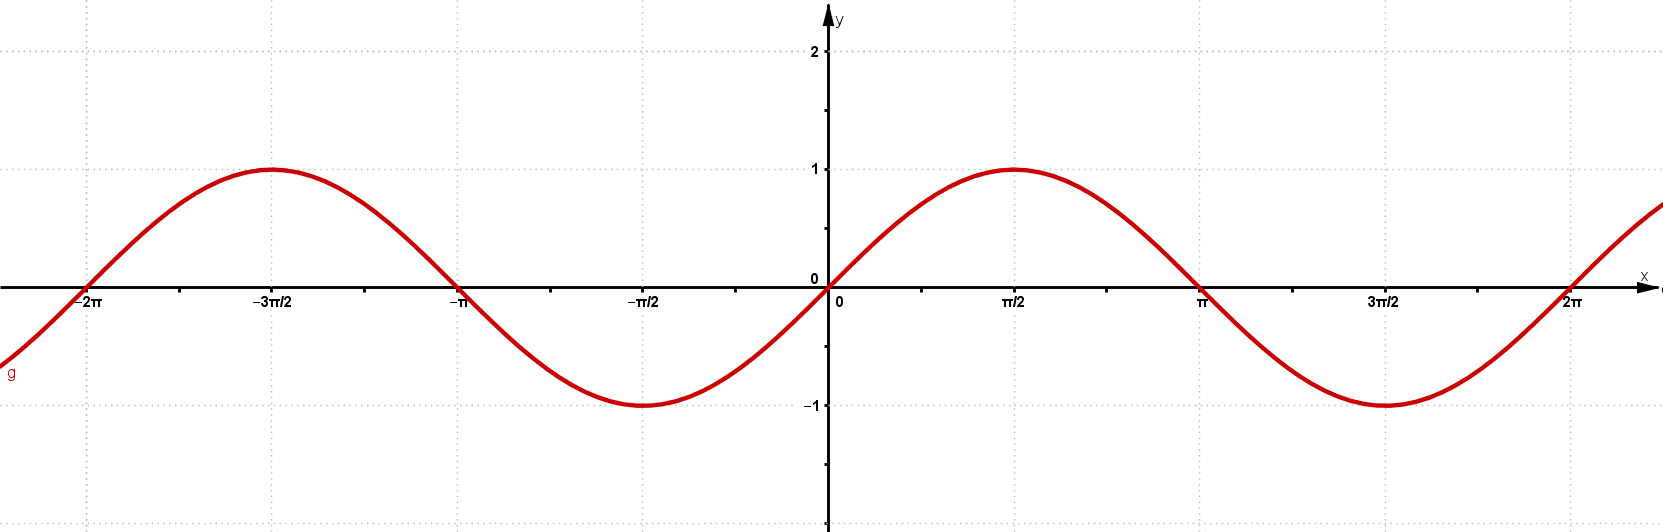
\includegraphics[width=0.95\textwidth]{sin.png}
\end{minipage}

\begin{minipage}{0.3\linewidth}
	\[ y=\cos (x)\\
	
	\begin{cases}
		Dom(\cos (x))= x \in \mathbb{R} \\ 
		Im(\cos (x))= [-1,1]\\
	\end{cases} \] 
\end{minipage}
\begin{minipage}{0.7\linewidth}
	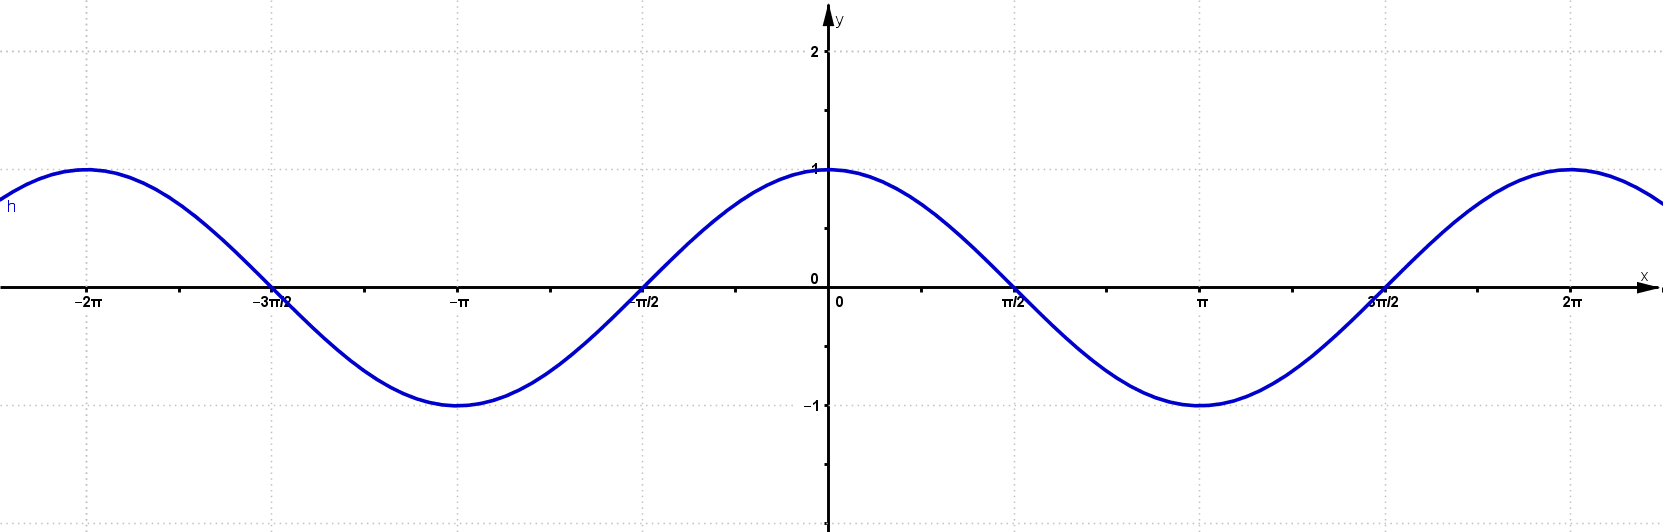
\includegraphics[width=0.95\textwidth]{cos.png}
\end{minipage}

En particular cabe destacar que las funciones trigonométricas se dicen que son $2\pi$ periódicas. ya que toma los mismos valores cada $2\pi$.\\

Una propiedad notoria del seno es que es una función \textbf{Impar}. En el sentido que $\sin(-x)=-\sin(x)$.

Osea que cambia de signo  para los x  negativos, comparado con los positivos.\\

Mientras que el coseno en una función \textbf{par}. En el sentido que $\cos (-x)=\cos (x)$

Osea que es igual tanto para los x positivos como para los negativos.\\

Por otro lado, 

\begin{minipage}{0.5\linewidth}
	\[ y=\tan (x)\\
	
	\begin{cases}
		Dom(\tan (x))= x \in \mathbb{R} - \lbrace x=\pi /2+n  & / n  \in \mathbb{N} \rbrace \\ 
		Im(\sin (x))= (-\infty,\infty)\\
	\end{cases} \] 
\end{minipage}
\begin{minipage}{0.5\linewidth}
	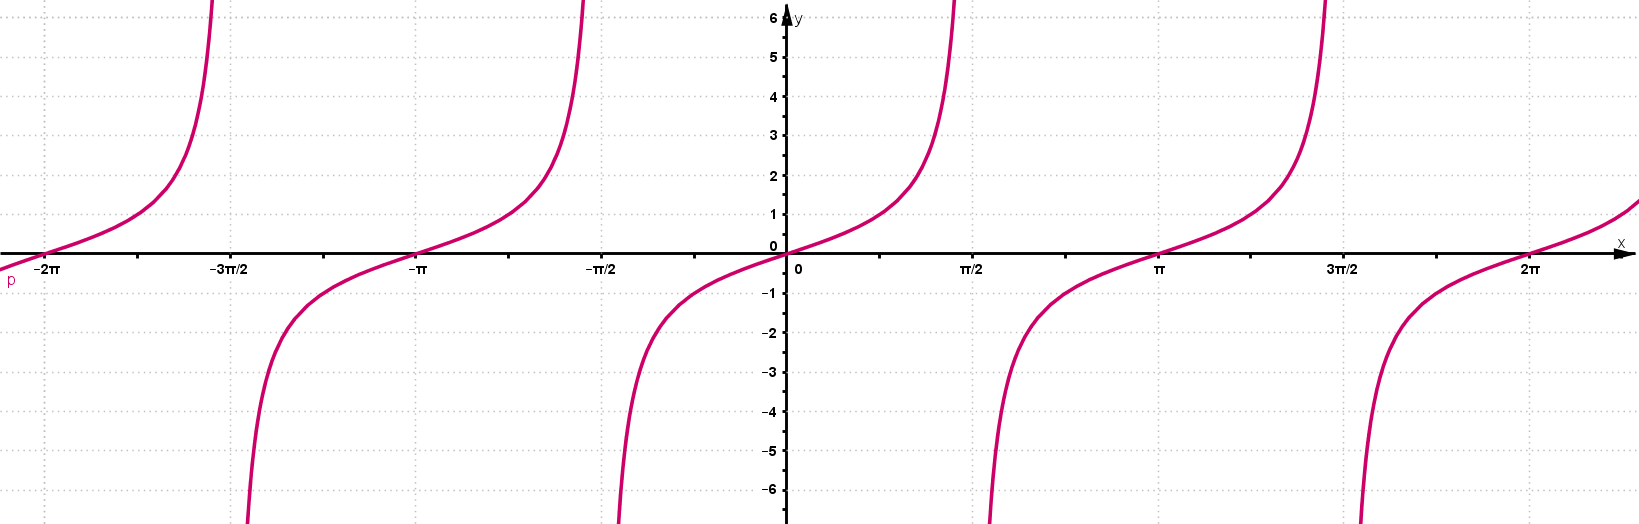
\includegraphics[width=.95\textwidth]{tan.png}
\end{minipage}

En general : %variar parametros de sen y cos : 

\[
y=A.\sin (w.x + \phi)+D
\]

\begin{center}
	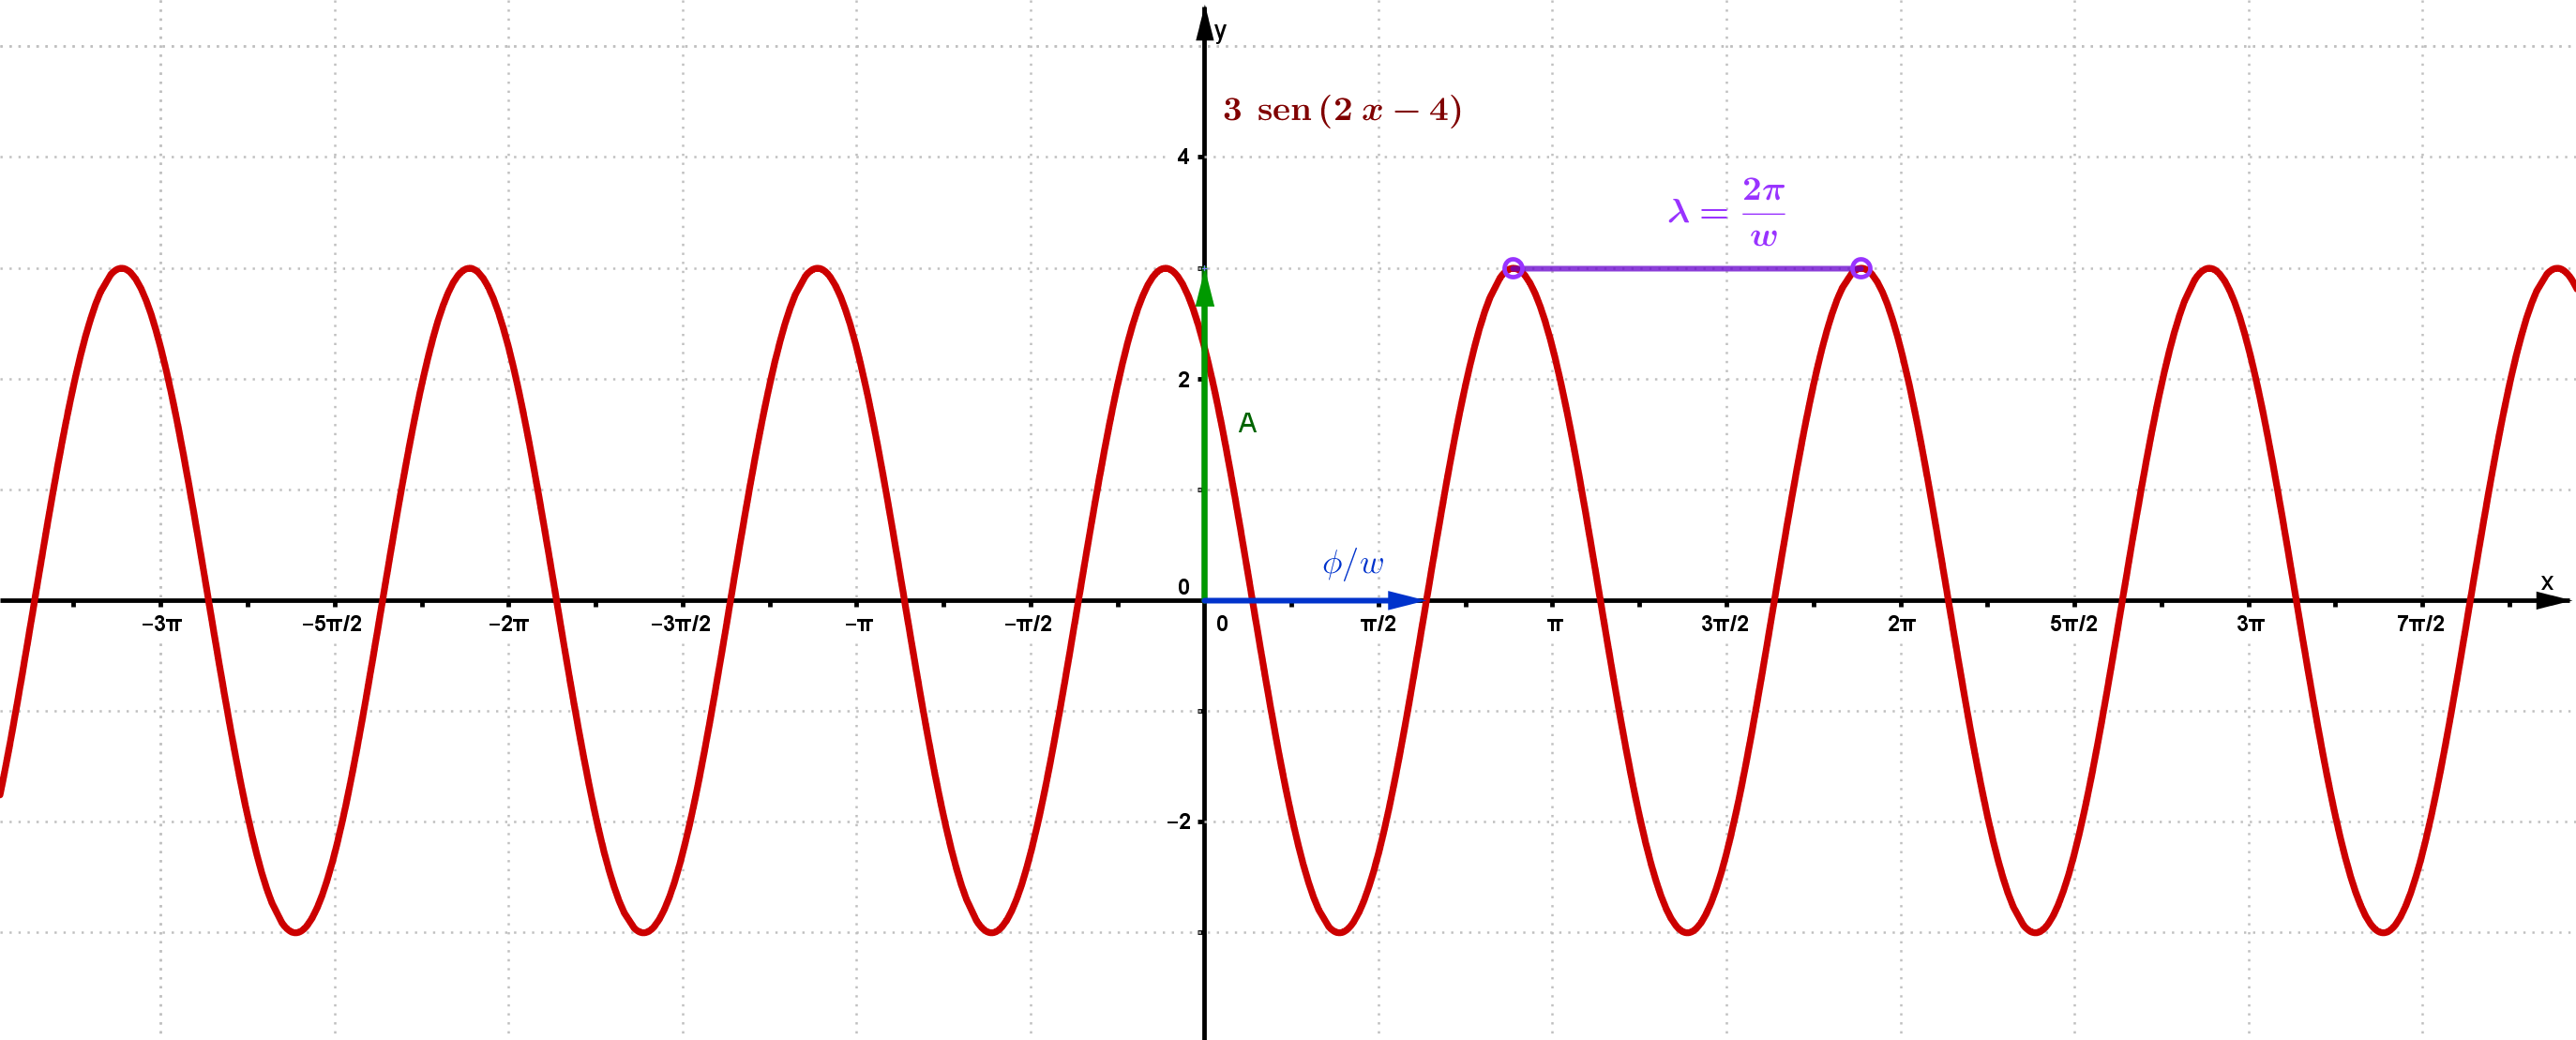
\includegraphics[width=0.85\linewidth]{singeneral.png}
\end{center}
\begin{flushright}
Donde $A$, $w$, $\phi$ y $D$ son constantes.
\end{flushright}
\begin{wrapfigure}{r}{0.25\textwidth}
	\begin{center}
		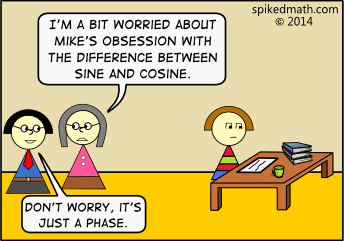
\includegraphics[width=\linewidth]{phase.png}
	\end{center}
\end{wrapfigure}
Donde \textquotedblleft $A$ \textquotedblright es llamada la amplitud, ya que cambia la amplitud de la oscilación del seno.
A \textquotedblleft $w$\textquotedblright se la llama frecuencia angular, ya que es la que modifica la frecuencia con la que el seno oscila (llega a un máximo, mínimo o pasa por $0$). También se define a $\lambda=\frac{2\pi}{w}$ como la longitud de onda, que es la distancia entre dos crestas o dos valles consecutivos.

A $\phi$ se lo llama fase o corrimiento, y es un factor que corre a la función hacia la izquierda o la derecha.

En particular se puede ver que si $\phi=\frac{w.\pi}{2}$, resulta que $A.\sin(w.x +\phi)=A.\cos(w.x)$.

Osea que el coseno y el seno son la misma función con una fase de diferencia.

\href{http://tube.geogebra.org/material/simple/id/686455}{\textcolor{blue}{Versión interactiva de seno y coseno como funciones de $x$}}

\section*{Funciones inversas}

Por ultimo, vamos a ver las funciones inversas del seno, el coseno y la tangente.

A una función $g(x)$ se la llama la inversa de $f(x)$, si $f(g(x))=x$. Es decir que si en $f(x)$ uno pone $g(x)$ en lugar de $x$, el resultado de toda la operación vuelve a dar $x$. \\

En este caso a $g(x)$ se la escribe como $f^{-1}(x)$, que es la notación que se le da a la inversa de la función $f$.\\

Por ejemplo: 

$\begin{cases}
f(x)= 10^x\\
g(x)= log(x)
\end{cases}
\Rightarrow  f(g(x))= 10^{log(x)}=x & \qquad \text{y también vale que} & \qquad g(f(x))=log(10^x)=x$.

En el ejemplo anterior: si $f(x)= 10^x  \Rightarrow f^{-1}(x)= log(x)$\\

Uso de las funciones inversas: 

si $f(x)=y \Rightarrow f^{-1}(f(x))=f^{-1}(y) \Leftrightarrow x=f^{-1}(y)$

ejemplo: $10^x=y \Rightarrow log(10^x)=log(y) \Leftrightarrow x=log(y)$\\

Las funciones inversas me da una forma de \textquotedblleft despejar x\textquotedblright cuando esta adentro de una función.

\textbf{Inversas de funciones trigonométricas:} 

\begin{minipage}{0.5\textwidth}
\centering
$a=\sin (b) \Rightarrow \arcsin(b)=a $ \\
$y=\arcsin(x)$\\ 
Rama principal:
$\begin{cases}
Dom(\arcsin(x))=\lbrace x \in \mathbb{R} / \quad x \in [-1,1] \rbrace \\
Im(\arcsin(x))=\lbrace y \in \mathbb{R} / \quad x \in [-\pi/2,\pi/2] \rbrace{}\\
\end{cases}
$
\end{minipage}
\begin{minipage}{0.5\textwidth}
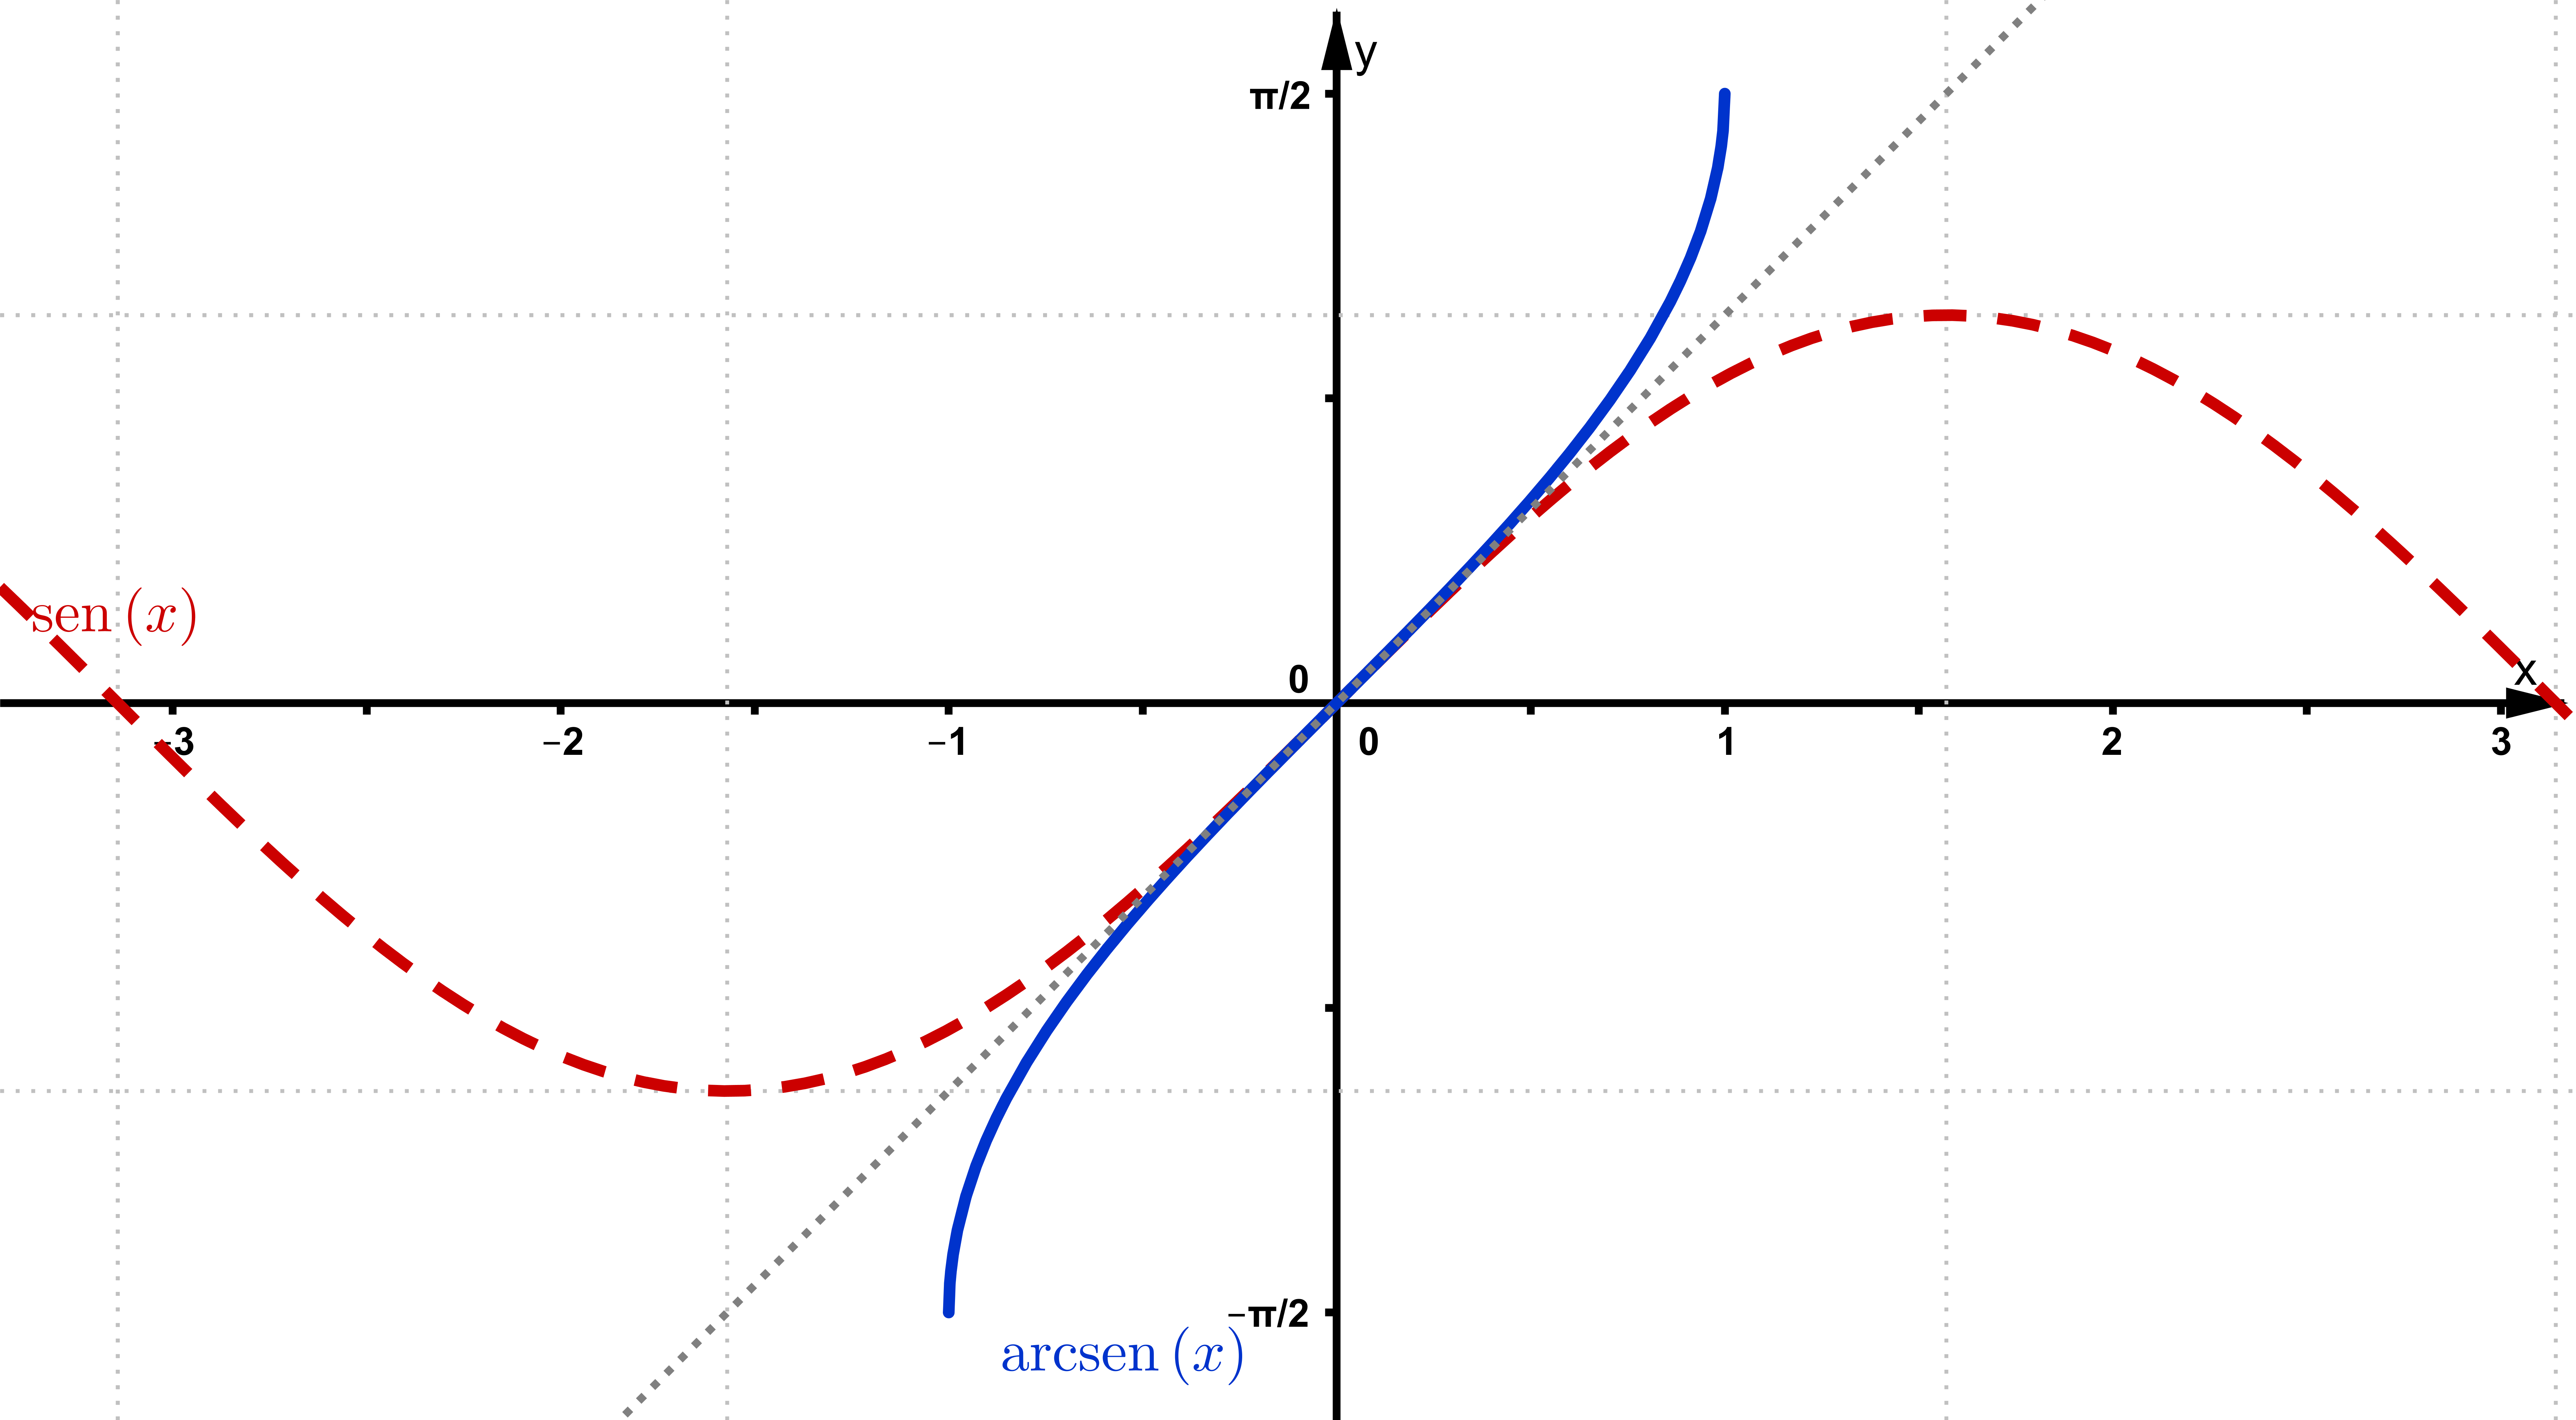
\includegraphics[width=\linewidth]{arcsen.png}
\begin{center}
	$y=\sin (x) $ en naranja $y=\arcsin(x)$ en azul. $y=x$ en gris.
\end{center}
\end{minipage}


\begin{minipage}{0.5\textwidth}
\centering
$a=\cos (b) \Rightarrow \arccos(b)=a $\\
$y=\arccos(x)$\\

Rama principal:

$\begin{cases}
Dom(y)=\lbrace x \in \mathbb{R} / \quad x \in [-1,1] \rbrace \\
Im(y)=\lbrace y \in \mathbb{R} / \quad x \in [0,\pi] \rbrace \\
\end{cases}
$
\end{minipage}
\begin{minipage}{0.5\textwidth}
	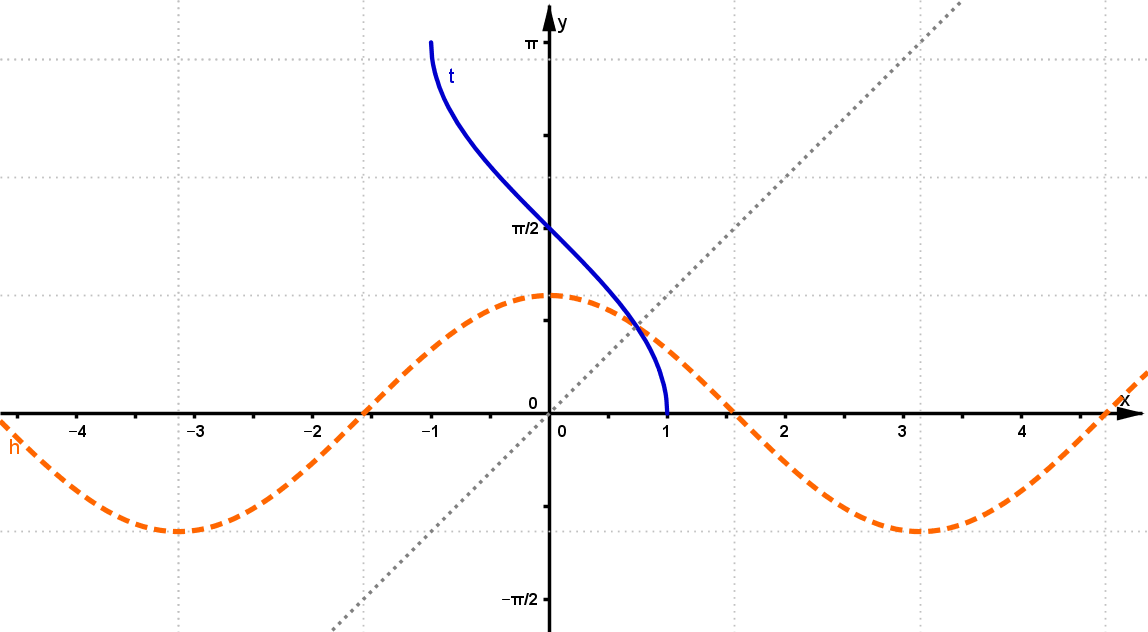
\includegraphics[width=\linewidth]{arccos.png}
	\begin{center}
		$y=\cos (x) $ en naranja $y=\arccos(x)$ en azul $y=x$ en gris.
	\end{center}
\end{minipage}

\begin{minipage}{0.5\textwidth}
	\centering
	$a=\tan(b) \Rightarrow \arctan(b)=a $ \\
	$y=\arctan(x)$\\
	Rama principal:
	$\begin{cases}
	Dom(y)=\lbrace x \in \mathbb{R} / \quad x \in [-\infty,\infty] \rbrace \\
	Im(y)=\lbrace y \in \mathbb{R} / \quad x \in [-\pi/2,\pi/2] \rbrace \\
	\end{cases}
	$
\end{minipage}
\begin{minipage}{0.5\textwidth}
	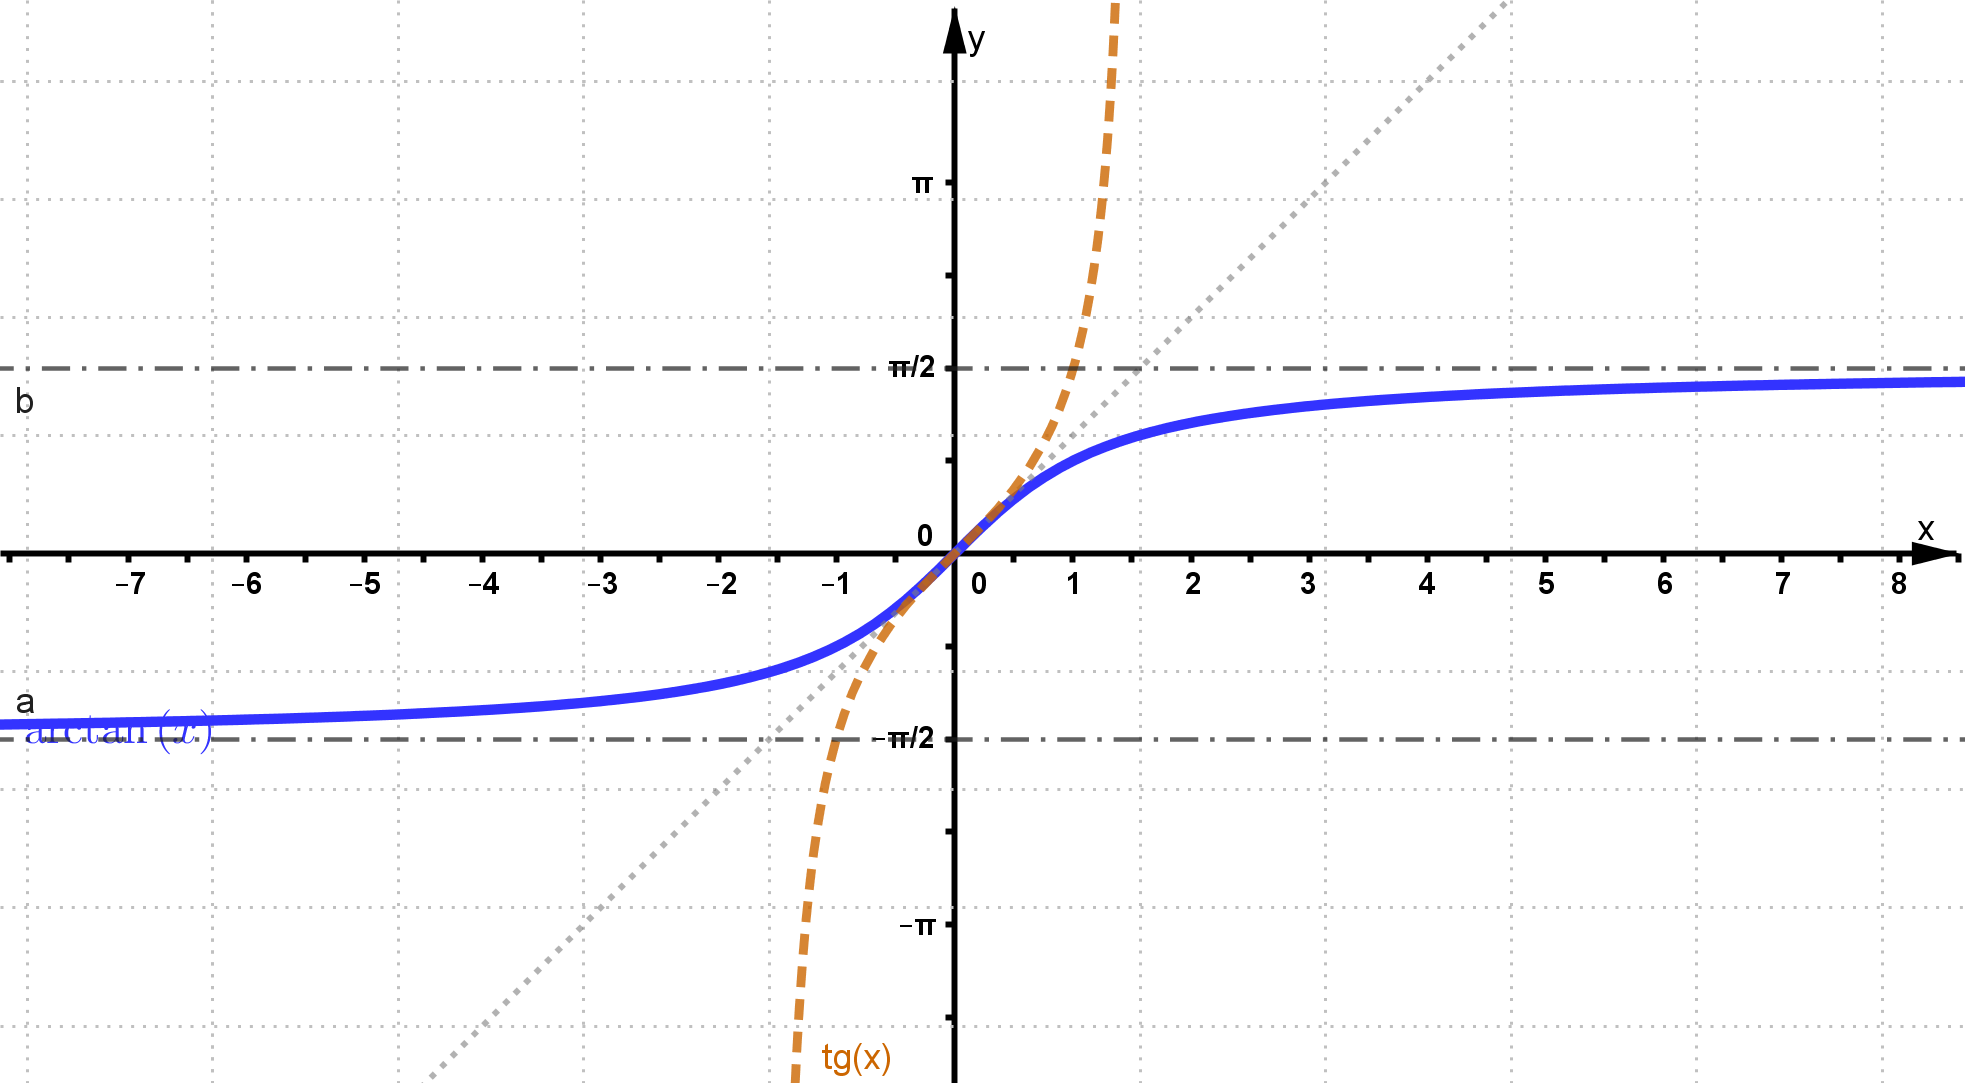
\includegraphics[width=\linewidth]{arctan.png}
	\begin{center}
		$y=\tan (x) $ en naranja $y=\arctan(x)$ en azul $y=x$ en gris.
	\end{center}
\end{minipage}

\section*{Relaciones entre las razones trigonométricas.}

Relación Pitagórica:

\[
\sin^2(x)+\cos^2(x)=1
\]

El seno y el coseno de la suma:

\[
\sin(\alpha+\beta)=\sin(\alpha)\cos(\beta) + \cos(\alpha)\sin(\beta)
\]
\[
\cos(\alpha+\beta)=\cos(\alpha)\cos(\beta) - \sin(\alpha)\sin(\beta)
\]

Estas propiedades son muy útiles y  valen siempre, sin importar el tipo de  problema.

Otra fácil de deducir es que $\tan(x)=\frac{\sin (x)}{\cos (x)}$.

Hay otra familia de funciones trigonométricas que se derivan a partir de estas tres:

\begin{itemize}
	\item  $\cosec (x)=\frac{1}{\sin (x)}$ .  'Cosecante'
	\item  $\sec (x)=\frac{1}{\cos (x)}$.  'Secante'
	\item  $\cot  (x)=\frac{1}{\tan (x)}=\frac{\cos (x)}{\sin(x)}$ . ' Cotangente'
\end{itemize}


\section*{Ejercicios}

Si se traban con algún ejercicio, pasen al siguiente, y vuelvan al ejercicio difícil mas tarde.\\

\textbf{TP:} Los que necesiten nota, pueden entregar esta guía de ejercicios resuelta como trabajo practico. Para aprobar el trabajo practico hace falta resolver(justificados) al menos el 70 por ciento de cada sección.

Los ejercicios con $\bigstar $ son obligatorios, menos el que tiene $\bigstar \bigstar$.


\section{Completar:}

%\begin{table*}[ht!]
\begin{center}
%\caption{Completar}
\label{completar}
\begin{tabular}{|l|c|c|c|c|c|c|c|c|c|c|c|c|c|c|c|c|c|}
	\hline
	Radianes & 0 & $\frac{\pi}{6} $ & $\frac{\pi}{4} $ & $\frac{\pi}{3} $ & $\frac{\pi}{2} $ & $1$ & $8\pi$ &  & & &   &   &  &  & \Ts \Bs \\ \hline
	Grados  &    &  &  & & &   &  & $300\degree$   & $150\degree$  & $90\degree$   & $30\degree$  & $45\degree$ &  $1\degree$ & $1250\degree$ & $210\degree$ \Ts \Bs     \\ \hline
\end{tabular}
%\end{table*}
%\caption{Completar}
%\label{completar}
%\begin{tabular}{|l|c|c|c|c|c|c|c|}
%\hline
%Radianes &  &  &   &   &  &  & \Ts \Bs \\ \hline
%Grados  & $300\degree$   & $150\degree$  & $90\degree$   & $30\degree$  & $45\degree$ &  $1\degree$ & $1250\degree$ \Ts \Bs     \\ \hline
%\end{tabular}
%%\end{table*}
\end{center}


\section{Resolver los siguientes triángulos rectángulos:}
\label{sec:rectangulos}

\begin{multicols}{2}
	\begin{tikzpicture}[thick]
	\coordinate (O) at (0,0);
	\coordinate (A) at (-4,0);
	\coordinate (B) at (0,-2);
	\draw (O)--(A)--(B)--cycle;
	
	\tkzLabelSegment[above=2pt](O,A){\textit{$a$}}
	\tkzLabelSegment[right=2pt](O,B){\textit{$b$}}
	\tkzLabelSegment[below left=2pt](A,B){\textit{$h$}}
	
	\tkzMarkRightAngle[fill=orange,size=0.5,opacity=.4](A,O,B)% square angle here
	\tkzLabelAngle[pos = -0.35](A,O,B){$\gamma$}
	
	\tkzMarkAngle[fill= orange,size=0.8cm,%
	opacity=.4](B,A,O)
	\tkzLabelAngle[pos = 0.6](B,A,O){$\alpha$}
	
	\tkzMarkAngle[fill= orange,size=0.7cm,%
	opacity=.4](O,B,A)
	\tkzLabelAngle[pos = 0.5](O,B,A){$\beta$}
	\end{tikzpicture}
	\begin{enumerate}
	\item $a=10cm$ $b=7cm$
	\item $h=11cm$ $a=9cm$
	\item $h=12cm$ $\sin (\alpha)=0,896$
	\item $a=5cm$ $\sin (\alpha)=0,5$%quedan 4 mas almenos
	\item $h=12$ $\cos(\alpha)=\tfrac{2}{3}$
	
\columnbreak

	\item $\bigstar$ $h=1$, calcular usando geometría $\sin(\alpha)$ y $\cos(\alpha)$ para $\alpha=30\degree & , 45\degree & , 60\degree$. 
%problema de la isla

\end{multicols}

	\item $\bigstar$ Suponiendo un rectángulo que tiene una diagonal de $55,88cm$ ($22 \quad \text{pulgadas}$), y la relación entre el lado $\overline{a}$ y el lado $\overline{b}$ es de  $16:9$ ($\frac{\overline{a}}{\overline{b}}=16/9$). ¿ Cuanto miden los lados $\overline{a}$ y $\overline{b}$?, ¿ y si la relación fuese $4:3$? Dibujar como serian los rectángulos. \label{itm:ratios}
Fíjense que aunque tengan la diagonal igual de larga, el área del rectángulo con $16:9$ es mayor al área del rectángulo con $4:3$.

	\item Sobre un círculo de 4 cm de radio se traza un ángulo central de 60°. Hallar el área del segmento circular comprendido entre la cuerda que une los extremos de los dos radios y su arco correspondiente.

\end{enumerate} 

\section{Calcular geometricamente los siguientes senos y cosenos}
\begin{tabular}{|l|c|c|c|c|c|}
	\hline
	Angulo & 0 & $\frac{\pi}{6} $ & $45\degree$ & $\frac{\pi}{3} $ & $\frac{\pi}{2} $   \Ts \Bs \\ \hline
	Seno  &    &  &  & & \Ts \Bs     \\ \hline
	Coseno &    &  &  & &  \Ts \Bs     \\ \hline
\end{tabular}


\section{Resolver los siguientes triangulos obtusos}

De los 6 valores posibles que se tiene el triangulo (3 lados y 3 ángulos). Dados 3 datos cualquiera (1 angulo y dos lados, 3 lados, 2 ángulos y un lado), el triangulo queda completamente determinado y se pueden hallar todos los valores restantes.

\begin{enumerate}
\begin{minipage}{0.45\linewidth}

\begin{tikzpicture}[thick]
	\coordinate (O) at (0,0);
	\coordinate (A) at (3.5,0);
	\coordinate (B) at (-1,3);
	\draw (O)--(A)--(B)--cycle;
	
	\node at (O) [below left=2pt]{$a$};
	\node at (A) [right=2pt]{$b$};
	\node at (B) [above left=2pt]{$c$};
	
	\tkzLabelSegment[below=2pt](O,A){}
	\tkzLabelSegment[left=2pt](O,B){}
	\tkzLabelSegment[above right=2pt](A,B){}
	
	\tkzMarkAngle[fill=orange,size=0.6,opacity=.4](A,O,B)% square angle here
	\tkzLabelAngle[pos = 0.35](A,O,B){$\hat{a}$}
	
	\tkzMarkAngle[fill= orange,size=0.8cm,%
	opacity=.4](B,A,O)
	\tkzLabelAngle[pos = 0.6](B,A,O){$\hat{b}$}
	
	\tkzMarkAngle[fill= orange,size=0.7cm,%
	opacity=.4](O,B,A)
	\tkzLabelAngle[pos = 0.5](O,B,A){$\hat{c}$}
\end{tikzpicture}

	\item  Verificar que los teoremas del seno y el coseno valen si tengo un triangulo con $\hat{a}=70\degree$, $\hat{b}=80\degree$, $\hat{c}=30$,  $\overline{ab}=7,62 cm$, $\overline{bc}=14,32cm$ ,$\overline{ca}=15cm$. Dibujar el triangulo. 
		
\end{minipage}
& $\qquad$
\begin{minipage}{0.45\linewidth}
	
		\item $\hat{a}=115\degree$, $\hat{b}=40\degree$, y $\overline{ac}=45cm$. Dibujar aproximadamente el triangulo y encontrar el valor de $x= \overline{bc}$.
		\item $\hat{c}=40\degree$,  $\overline{ac}=30cm$ y $\overline{ab}=20cm$ . Dibujar aproximadamente el triangulo y encontrar el valor de $x= \hat{b}$.
		\item $\hat{a}=30\degree$,  $\overline{ac}=15cm$ y $\overline{ab}=10cm$ . Dibujar aproximadamente el triangulo y encontrar el valor de $x= \overline{bc}$.
		\item $\overline{ab}=10cm$,  $\overline{ac}=7cm$ y $\overline{bc}=8cm$ . Dibujar aproximadamente el triangulo y encontrar el valor de $x= \hat{c}$.
		\item $\hat{a}=60\degree$, $\hat{b}=70\degree$, y $\overline{ac}=20m$. Dibujar aproximadamente el triangulo y resolverlo (hallar todos los valores restantes).
		\item $\overline{ab}=28m$,  $\hat{c}=43\degree$ y $\overline{ac}=27m$ . Dibujar aproximadamente el triangulo y encontrar el valor de $x= \hat{c}$.
		
		
\end{minipage}
\end{enumerate}

\section{Problemas}

\begin{enumerate}

	\item ¿ Cual es el angulo de elevación del sol cuando un mástil de $24m$ proyecta una sombra de $16m$?
	\item ¿ Cual es la altura de una antena si una persona que se encuentra a $250m$ de su base, observa su punta bajo un angulo de $22\degree$?
	\item ¿ Cual es el área de un pentágono regular de $40cm$ de perímetro?
	\item ¿ Cual es el área de un triangulo isósceles, cuya base mide $18cm$ y el angulo opuesto a ella mide $34\degree 50'$?
	\item El perímetro de un triangulo isósceles es de $26cm$ y su base mide $10cm$. ¿ Cual es el valor de sus ángulos interiores?

\end{enumerate} 

\section{Deducir las siguientes propiedades}
Pensando en la interpretación que vimos del seno y el coseno para un circulo de radio 1, deducir la siguientes propiedades:

Si $0\leq \alpha \leq \pi/2$

\begin{enumerate}
\begin{multicols}{2}
	\item $\sin(\pi - \alpha)=\sin(\alpha)$
	\item \bigstar $\sin(\frac{3}{2}\pi - \alpha)=-\sin(\alpha)$
	\item $\sin(2\pi - \alpha)=-\sin(\alpha)$
\columnbreak
	\item $\cos(\pi - \alpha)=-\cos(\alpha)$
	\item \bigstar $\cos(\frac{3}{2}\pi - \alpha)=-\cos(\alpha)$
	\item $\cos(2\pi - \alpha)=\cos(\alpha)$
\end{multicols}
\end{enumerate}

\section{Decidir Verdadero o Falso y justificar}

\begin{enumerate}
\begin{multicols}{2}
	\item $\forall x \backslash x \in \mathbb{R} & \qquad \cos(x)\geqslant \sin(x)$
	\item $\forall x \backslash x \in \mathbb{R} & \qquad 0\leqslant \sin^2(x)\leqslant 2$
	\item $\forall x \backslash x \in \mathbb{R} & \qquad \cos(x)\geqslant \sin(x)$
	\item $\forall x \backslash x \in \mathbb{R} & \qquad \cos^2(x)+ \sin^2(x)\leqslant 1$
	\columnbreak
	\item $\forall x \backslash x \in \mathbb{R} & \qquad \tan(x) \in \mathbb{R}$
	\item $\exists x \backslash x \in \mathbb{R} & \qquad \sin(x)>2$
	\item La función seno es Par.
	\item La función seno es Impar.
\end{multicols}
\end{enumerate}


\section{Gráficos:}
\begin{enumerate}
	\begin{multicols}{2}
	
	
	\item $y=\sin(x)$, $y=\cos(x)$, $y=\tan(x)$
	\item $\bigstar$ $y=\sin(x+\pi/2)$, $y=\cos(x-\pi/2)$
	\item $y=2\sin(x+\pi)$
	\item $y=\cos(x)+1$
	\item $y=-1.\cos(x+\pi/2)$
	\item $\bigstar$ $y=\sin(2x)$
	\item $y=2.\cos(\frac{x}{2})$
	\item $y=-3.\sin(\frac{\pi}{2}.x)$%poner un par mas de estos
	
	\columnbreak
	
	\item Hallar y graficar la formula de una función de la forma $f(x)=A\sin(wx)$ que cumpla:
	\item[a.] $\bigstar$ Periodo $=\pi$, y  Máximo $=0,7$.
	\item[b.] $\bigstar$ $Im(f)=[-5,5]$ y realiza tres ciclos completos en $[0,2\pi]$.\\

\begin{center}
		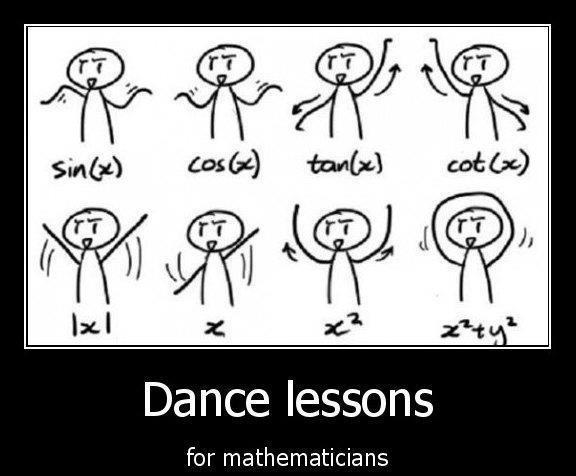
\includegraphics[width=0.36\textwidth]{dance.jpg}
		\label{fig:dance}
\end{center}

	\end{multicols}
\end{enumerate}

\section{Demostrar}
$\bigstar \bigstar$ $tg(\alpha)=a \Rightarrow \vert cos(\alpha).sen(\alpha)\vert =\frac{\vert a \vert}{a^2+1}$

\section{Demostrar cada una de las siguientes identidades trigonométricas}
\label{demostraciones}

\begin{multicols}{2}%ver restricciones de u
\begin{enumerate}
	
	\item  $ \sin^2(u)+cos^2(u)=1 $
	
	\item  $ tg(u)=\frac{\sin(u)}{cos(u)} $
	
	\item $cos^2(\alpha)-\sin^2(\alpha)=1-2.\sin^2(\alpha)$
	
	\item $\frac{cos(\alpha)}{cotg(\alpha)}=\sin(\alpha)$
	
	\item  $ \sin(u).cosec(u)=1 $
	
	\item  $ cos(u).sec(u)=1 $
	
	\item $\bigstar$ $\sin(\alpha-\beta)=\sin(\alpha)\cos(\beta) - \cos(\alpha)\sin(\beta)$
	
\columnbreak 
	 
	\item $\cos(\alpha-\beta)=\cos(\alpha)\cos(\beta) + \sin(\alpha)\sin(\beta)$
	
	\item $\cos(2.\alpha)=\cos^2(\alpha) - \sin^2(\alpha)$
	
	\item $\bigstar$ $\sin(2.\alpha)=2.\sin(\alpha)\cos(\alpha)$

	\item $\bigstar$ $\sin(\alpha)+\sin(\beta)=2.\sin(\frac{\alpha+\beta}{2})\cos(\frac{\alpha-\beta}{2})$
	
	\item $\sin(\alpha).\sin(\beta)=\frac{1}{2}[\sin(\alpha-\beta)-cos(\alpha+\beta)]$
	
	\item  $ tg(u).cotg(u) $
	
	\item $\sec(x)-\cos(x)=\tan(x).\sin(x)$
	
	\item  $ 1+tg^2(u)=\frac{1}{cos^2(u)}=sec^2(u) $
	
	\item  $ 1+cotg^2(u)=\frac{1}{\sin^2(u)}=cosec^2(u) $

\end{enumerate}
\end{multicols}

\section{Resolver las ecuaciones }
\label{ecuaciones}
Hallar $x/ \quad 0\leq x < 2\pi$ que verifica las siguientes ecuaciones.

\begin{multicols}{2}%ver restricciones de u

\begin{enumerate}

	\item  $\sin (x) = \cos(x) $
	\item $1-\cos^2(x)=0,25$
	\item  $2\sin(x)=cosec(x)$
	\item $4\cos^5(x)-3cos^3(x)=0$
	\item  $ cos^2(x)=cos(x) $
	\item $\sin(2x)+\sin(4x)=0$

%poner la suma y resta de cos y \sin
\columnbreak 

	\item $\tan (x)+\cot(x)=\frac{2}{cos(x)}$
	\item $\sin^2(x)-\sin(x)=0$
	\item  $ \sin(x)+tg(x)=0 $
	\item $4\sin^2(x)-8\sin(x)+3=0$
	\item $sec(4x)=1$

\end{enumerate}
\end{multicols}

%\section{Ejemplo de Aplicación}
%una persona tiene una pulsacion de ...
%una guitarra tiene se toda un nota LA (440hz). cuantos nodos tiene la cuerda... cada cuanto llega a un minimo.. velocidad del sonido..\\
%los rayos x viajan a una velocidad de .. y tiene una longitud de onda de....

\rule[2ex]{\textwidth}{2pt}


%gifsicle --unoptimize animated.gif | convert - frame-%d.png
%\animategraphics[loop,autoplay]{12}{frame-}{0}{99}
\section*{Extra}

\begin{itemize}

	\item Sobre el ejercicio \ref{sec:rectangulos}.\ref{itm:ratios}: Las relación $16:9$ es la que se utiliza actualmente en los televisores HD y en los monitores, Mientras que la relación $4:3$ es la que se usaba antiguamente. Por eso los televisores viejos se ven mas cuadrados. 
	Un televisor viejo de $20$ pulgadas y uno nuevo, tienen la diagonal de la misma longitud, pero uno se ve mas cuadrado que el otro, e incluso tienen diferente área. 
	
	
	\item \textbf{Triángulos que no suman $180\degree$:} Toda la geometría que vieron hasta ahora (desde la primaria) cae dentro de una rama de la geometría llamada geometría Eulidea o plana (en honor a Euclides).	
		\begin{minipage}{0.6\textwidth}
		Sin embargo existen otros tipos de geometrías, en las cuales pasan cosas a las que no estamos acostumbrados.
		Por ejemplo que dos rectas paralelas se toquen, que la distancia mas corta entre dos puntos no sea la recta que los une, o que la suma  de los ángulos internos de un triangulo sumen mas o menos de 180 grados.
		Estas geometrías se llaman geometrías de Riemman o curvas (En honor a Riemman, discípulo de Gauss).
		
		Por ejemplo, dibujar un triangulo que empiece en el polo de la tierra y siga dos latitudes, arma un triangulo cuyos ángulos internos suman mas de $180\degree$.
		\end{minipage}
		\begin{minipage}{0.4\textwidth}
			\begin{center}
				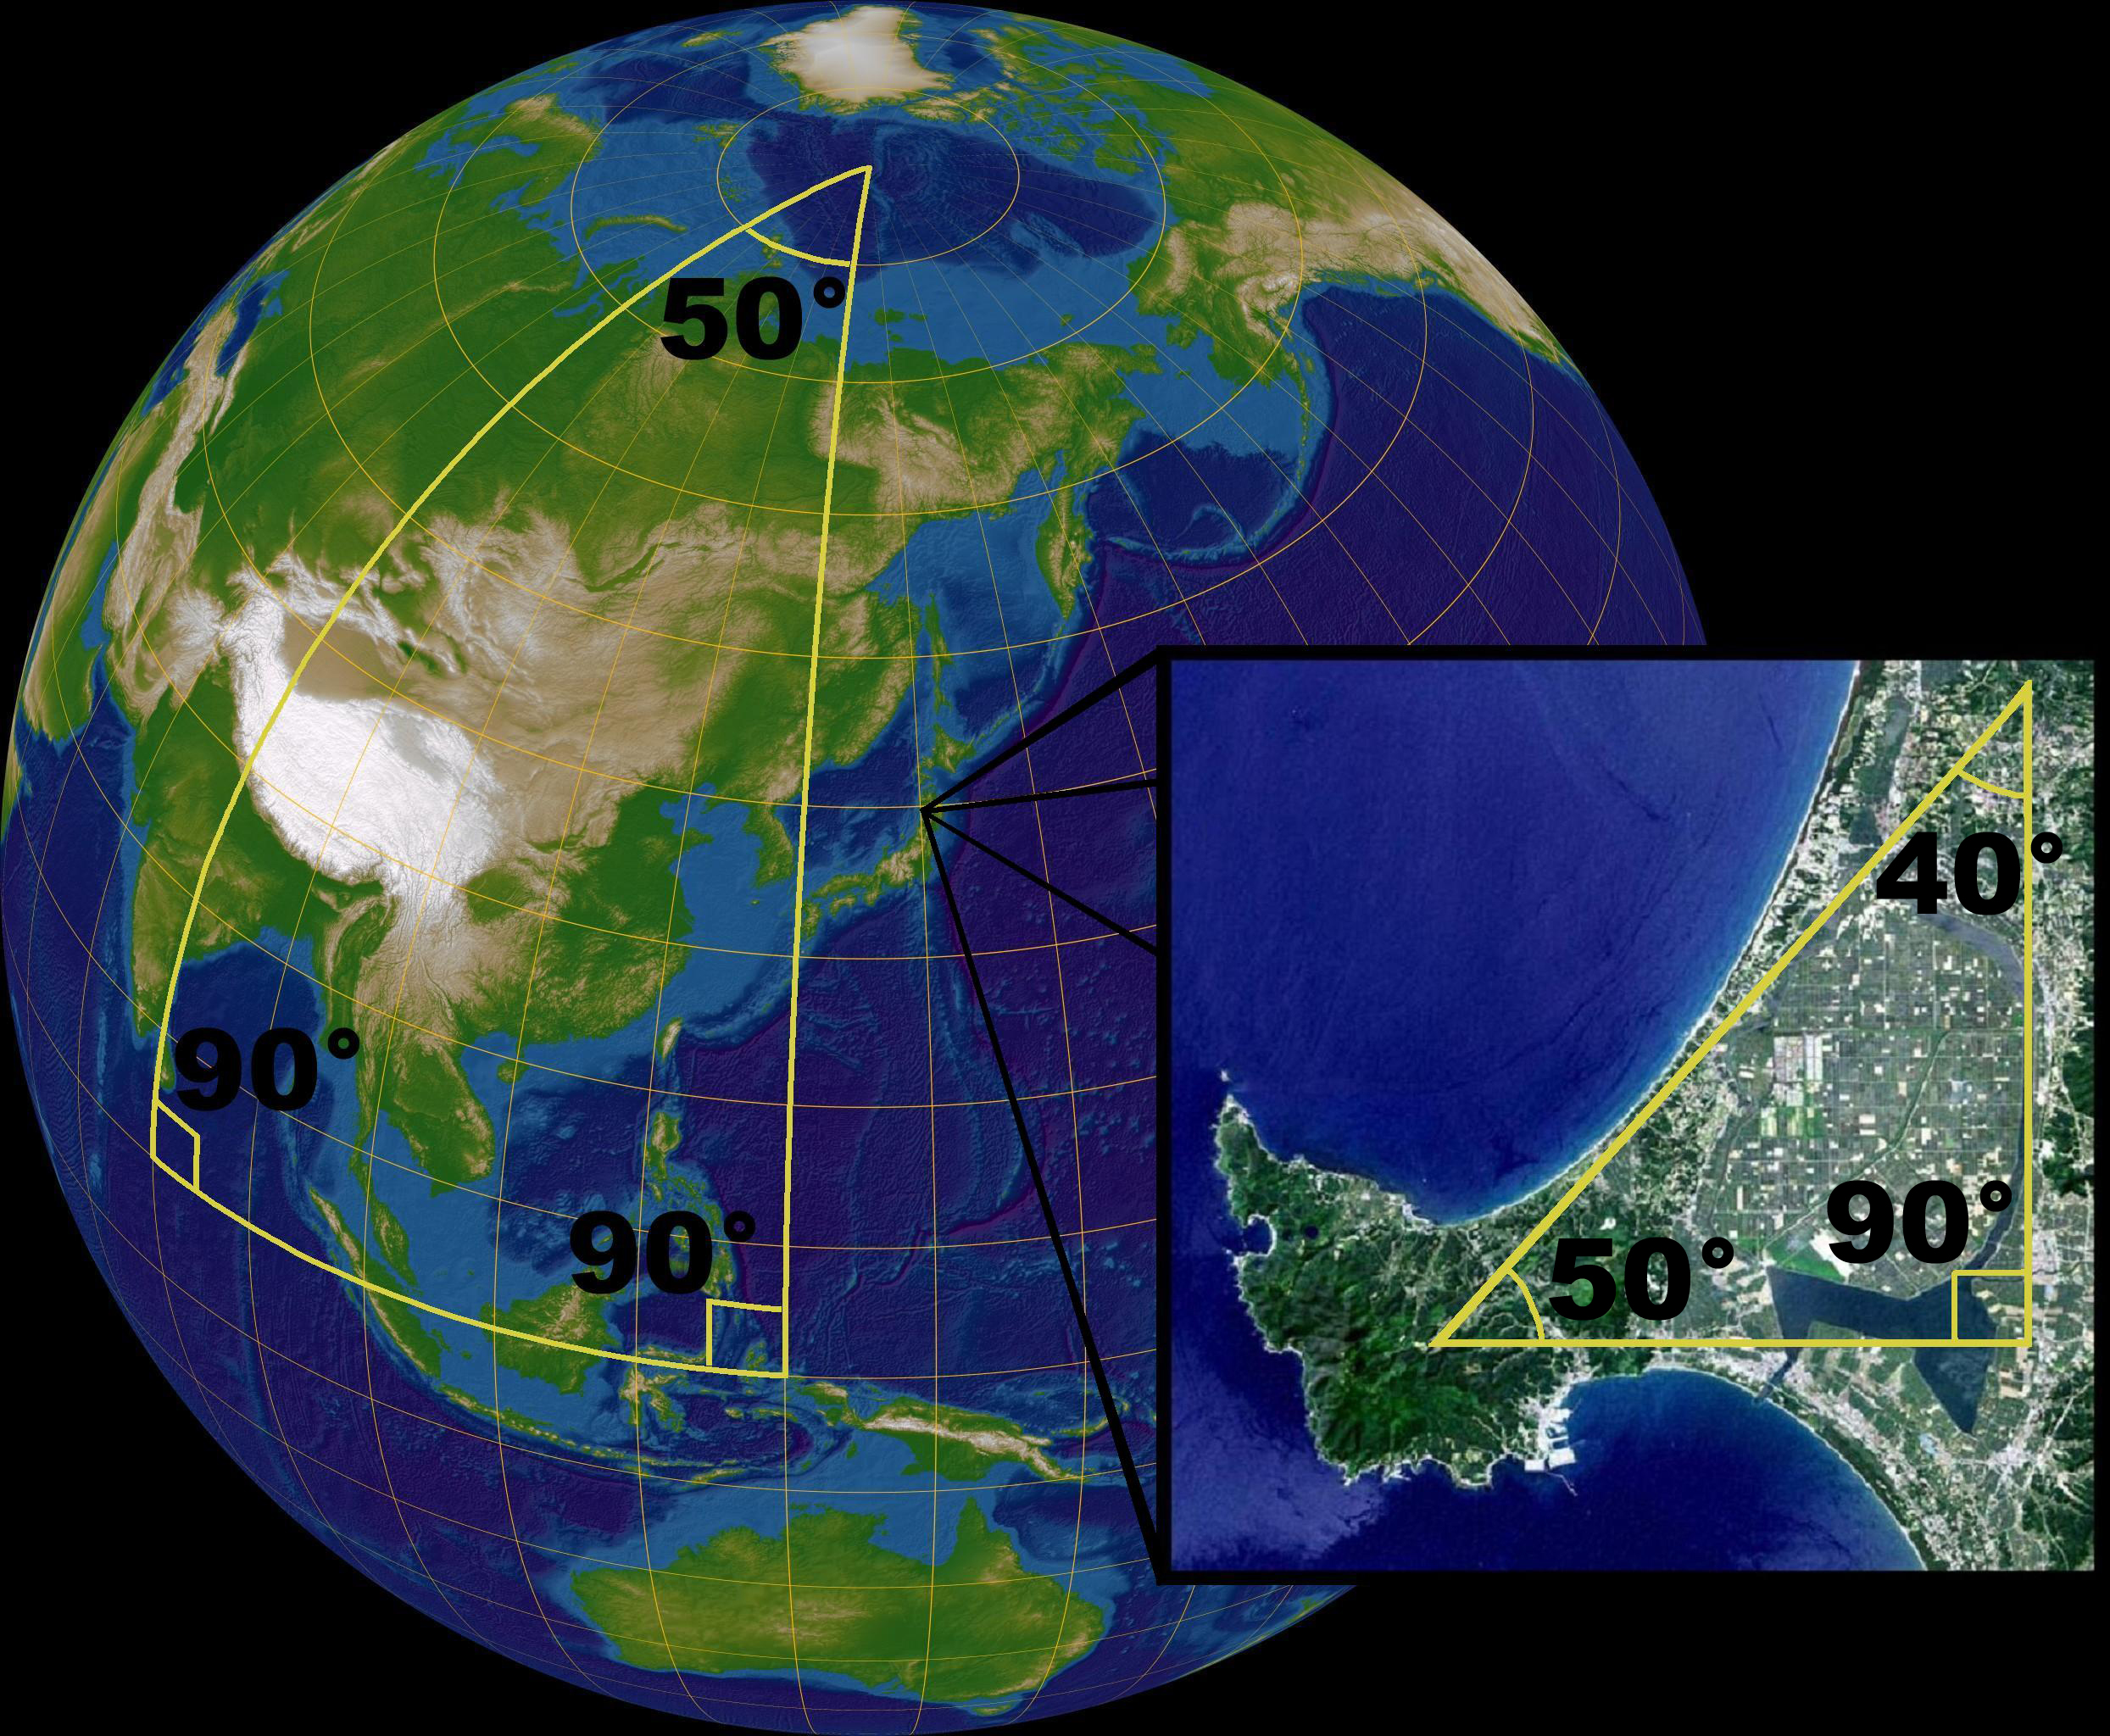
\includegraphics[width=0.95\linewidth]{esphtri.jpg}
			\end{center}
		\end{minipage}
		
	

	\item \href{http://tinyurl.com/orl4bqw}{\textcolor{blue}{El Triangulo de Penrose}}. Uno de tantos \textquotedblleft  objetos imposibles \textquotedblright :

\begin{minipage}{0,5\linewidth}
\begin{center}
	\begin{tikzpicture}[scale=0.5, line join=bevel]
	% \a and \b are two macros defining characteristic
	% dimensions of the Penrose triangle.		
	\pgfmathsetmacro{\a}{2.5}
	\pgfmathsetmacro{\b}{0.9}
	
	\tikzset{%
		apply style/.code     = {\tikzset{#1}},
		triangle_edges/.style = {thick,draw=black}
	}
	
	\foreach \theta/\facestyle in {%
		0/{triangle_edges, fill = gray!50},
		120/{triangle_edges, fill = gray!25},
		240/{triangle_edges, fill = gray!90}%
	}{
	\begin{scope}[rotate=\theta]
	\draw[apply style/.expand once=\facestyle]
	({-sqrt(3)/2*\a},{-0.5*\a})                     --
	++(-\b,0)                                       --
	({0.5*\b},{\a+3*sqrt(3)/2*\b})                -- % higher point	
	({sqrt(3)/2*\a+2.5*\b},{-.5*\a-sqrt(3)/2*\b}) -- % rightmost point
	++({-.5*\b},-{sqrt(3)/2*\b})                    -- % lower point
	({0.5*\b},{\a+sqrt(3)/2*\b})                  --
	cycle;
	\end{scope}
}	
\end{tikzpicture}

Triangulo de Penrose.
\end{center}
\end{minipage}
\begin{minipage}{0,5\linewidth}
	\begin{center}
		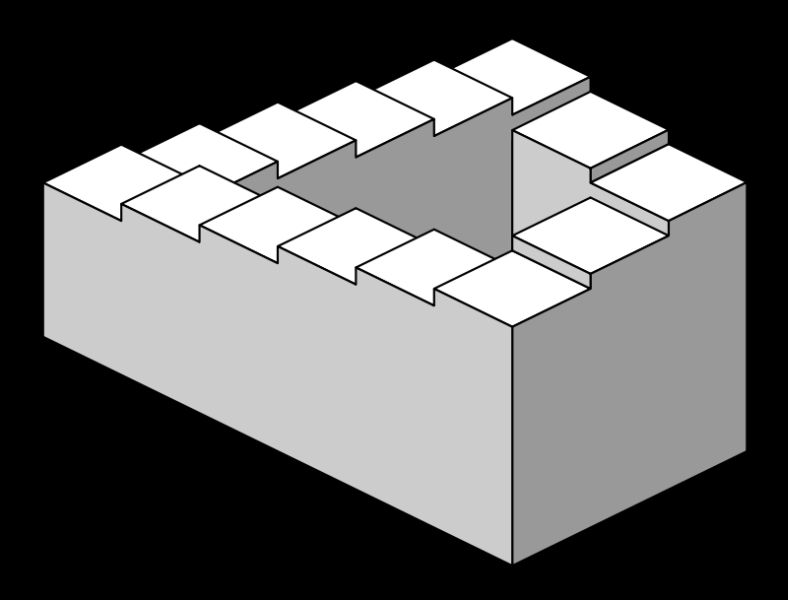
\includegraphics[width=0.55\textwidth]{penrosesairs.jpg}
		
		Escaleras de Penrose.
	\end{center}
\end{minipage}	

\end{itemize}



\begin{tikzpicture}[scale=2]
\tikzstyle{ann} = [draw,ultra thick, fill=blue!20,right]{
	\node[regular polygon,regular polygon sides=5] {};\\
	
};
\end{tikzpicture}

%\begin{tikzpicture}
%\begin{axis}[ domain=-360:360 , samples=80 ,
%width=10cm , height=7cm , xmax=800]
%\addplot [color=red , mark=x] coordinates {
%( -200 , -1)
%( -133 , -1.2)
%( -66 , -2)
%(0 , -2.5)
%(66 , -4)
%(133 , -5)
%(200 , -7)
%};
%\addplot[color = blue] {sin(x)};
%\addplot[color = green] {-4+ x/90+ cos(x*2)};
%\end{axis}
%\end{tikzpicture}


\definecolor{zzttqq}{rgb}{0.6,0.2,0.}
\begin{tikzpicture}[line cap=round,line join=round,>=triangle 45,x=1.0cm,y=1.0cm]
\clip(-8.263715031368294,-0.8466907429406771) rectangle (7.698985586095146,7.274193662097544);
\fill[color=zzttqq,fill=zzttqq,fill opacity=0.1] (-2.,0.) -- (2.,0.) -- (3.23606797749979,3.804226065180613) -- (0.,6.155367074350506) -- (-3.2360679774997894,3.8042260651806146) -- cycle;
\draw [color=zzttqq] (-2.,0.)-- (2.,0.);
\draw [color=zzttqq] (2.,0.)-- (3.23606797749979,3.804226065180613);
\draw [color=zzttqq] (3.23606797749979,3.804226065180613)-- (0.,6.155367074350506);
\draw [color=zzttqq] (0.,6.155367074350506)-- (-3.2360679774997894,3.8042260651806146);
\draw [color=zzttqq] (-3.2360679774997894,3.8042260651806146)-- (-2.,0.);
\draw [line width=1.6pt,dash pattern=on 2pt off 2pt] (0.,3.077683537175253)-- (0.,0.);
\draw [line width=1.2pt,dash pattern=on 2pt off 2pt] (0.,3.077683537175253)-- (2.,0.);
\end{tikzpicture}

%\bibliographystyle{plain}
%\bibliography{references}

%
%\newpage
%
%\section*{Resultados}
%\begin{enumerate}
%\item
%\begin{enumerate}


\end{document}